\documentclass[12pt]{article}
\usepackage{amsthm,amssymb,amsmath,amsfonts}
\usepackage[a4paper, top=25mm, bottom=30mm, left=25mm, right=25mm]{geometry}
\usepackage[pagebackref=false,colorlinks,linkcolor=black,citecolor=black]{hyperref}
\usepackage[nameinlink]{cleveref}
 \AtBeginDocument{%
    \crefname{equation}{برابری}{equations}%
    \crefname{chapter}{فصل}{chapters}%
    \crefname{section}{بخش}{sections}%
    \crefname{appendix}{پیوست}{appendices}%
    \crefname{enumi}{مورد}{items}%
    \crefname{footnote}{زیرنویس}{footnotes}%
    \crefname{figure}{شکل}{figures}%
    \crefname{table}{جدول}{tables}%
    \crefname{theorem}{قضیه}{theorems}%
    \crefname{lemma}{لم}{lemmas}%
    \crefname{corollary}{نتیجه}{corollaries}%
    \crefname{proposition}{گزاره}{propositions}%
    \crefname{definition}{تعریف}{definitions}%
    \crefname{result}{نتیجه}{results}%
    \crefname{example}{مثال}{examples}%
    \crefname{remark}{نکته}{remarks}%
    \crefname{note}{یادداشت}{notes}%
    \crefname{observation}{مشاهده}{observations}%
    \crefname{algorithm}{الگوریتم}{algorithms}%
    \crefname{cproof}{برهان}{cproofs}%
}

\usepackage{tikz}
\usepackage{graphicx}
\usepackage{color}

\usepackage{setspace}
\doublespacing

\usepackage{titletoc}
\usepackage{tocloft}
\usepackage{enumitem}

\usepackage{algorithm}
% \usepackage[noend]{algpseudocode}
\usepackage[noend]{algorithmic}
\renewcommand{\algorithmicrequire}{\textbf{Input:}}
\renewcommand{\algorithmicensure}{\textbf{Output:}}

\usepackage{tabularx}
\makeatletter
\newcommand{\multiline}[1]{%
  \begin{tabularx}{\dimexpr\linewidth-\ALG@thistlm}[t]{@{}X@{}}
    #1
  \end{tabularx}
}
\makeatother

\usepackage{float}
\usepackage{verbatim}
\makeindex
\usepackage{sectsty}
\usepackage{xepersian}
\SepMark{-}
\settextfont[Scale=1.2,Path=fonts/,BoldFont=B Nazanin Bold.ttf]{B Nazanin.ttf}
\setlatintextfont{Times New Roman}
\renewcommand{\labelitemi}{$\bullet$}

\theoremstyle{definition}
\newtheorem{definition}{تعریف}[section]
\newtheorem{remark}[definition]{نکته}
\newtheorem{note}[definition]{یادداشت}
\newtheorem{example}[definition]{نمونه}
\newtheorem{question}[definition]{سوال}
\newtheorem{remember}[definition]{یاداوری}
\newtheorem{observation}[definition]{مشاهده}
\theoremstyle{theorem}
\newtheorem{theorem}[definition]{قضیه}
\newtheorem{lemma}[definition]{لم}
\newtheorem{proposition}[definition]{گزاره}
\newtheorem{corollary}[definition]{نتیجه}
\newtheorem*{cproof}{برهان}



\begin{document}
\fontsize{12pt}{14pt}\selectfont

\begin{minipage}{0.1\textwidth}

\end{minipage}%
\hfill%
\begin{minipage}{0.6\textwidth}\centering
\fontsize{10pt}{10pt}\selectfont
به نام خداوند \\
تئوری یادگیری ماشین \\
دکتر سیدصالحی\\
جلسه سوم
 \\
\vspace{0.25cm}
\begingroup
\fontsize{8pt}{8pt}\selectfont
دانشکده ریاضی و علوم کامپیوتر \\
اسفند ماه 1402\\
\endgroup
\end{minipage}%
\hfill%
\begin{minipage}{0.1\textwidth}
\end{minipage}

\vspace{0.5cm}

\noindent\rule{\textwidth}{1pt}

\section{ مسئله $Classification$}

مسئله $Classification$ یا طبقه‌بندی، یکی از مسائل اصلی در یادگیری ماشین و داده‌کاوی است که هدف آن تخصیص دادن هر نمونه یا داده به یکی از دسته‌ها یا کلاس‌های مشخص است بر اساس ویژگی‌ها یا خصوصیات آن نمونه. به زبان ساده‌تر، در یک مسئله طبقه‌بندی، ما می‌خواهیم پیش‌بینی کنیم که یک مورد خاص به کدام دسته تعلق دارد. به عنوان مثال، طبقه‌بندی ایمیل‌ها به «اسپم» یا «غیراسپم»، تشخیص اینکه یک تصویر حاوی گربه است یا سگ، یا تعیین اینکه یک تراکنش مالی مشکوک به تقلب است یا خیر، همگی از مثال‌هایی برای مسائل طبقه‌بندی هستند.

در طبقه‌بندی، مجموعه آموزشی یا $Training\:Set$ شامل داده‌هایی است که برای آموزش مدل یادگیری ماشین استفاده می‌شوند. این داده‌ها شامل نمونه‌هایی با ویژگی‌های مشخص هستند که هر کدام به یکی از کلاس‌های مورد نظر ما مربوط می‌شوند. هر نمونه در این مجموعه دارای یک برچسب یا کلاس معین است که مشخص می‌کند به کدام دسته تعلق دارد. 

دو نوع اصلی مسائل طبقه‌بندی در یادگیری ماشین عبارت اند از: طبقه‌بندی دودویی (باینری) و طبقه‌بندی چندکلاسه.

- در حالت دو کلاسی (باینری)، خروجی‌ها به صورت \(y \in \{0, 1\}\) نمایش داده می‌شوند. به این معنی که هر نمونه می‌تواند به یکی از دو کلاس موجود تعلق داشته باشد، معمولاً 0 نمایانگر کلاس منفی و 1 نمایانگر کلاس مثبت است. به عنوان مثال، در تشخیص ایمیل‌های اسپم، یک ایمیل می‌تواند اسپم (1) یا غیراسپم (0) باشد. 

- در حالت چند کلاسی، خروجی‌ها اغلب به صورت بردارهایی از اعداد 0 و 1 نمایش داده می‌شوند که به آنها بردارهای یک‌داغ یا $one-hot\:vectors$ گفته می‌شود. برای مثال، \(y = [0, 1, 0, 0, 0]\) نشان می‌دهد که نمونه به کلاس دوم تعلق دارد ( کلاس‌ها از 1 تا \(K\) شماره‌گذاری شده‌اند، و در این مثال \(K\geq5\)). در این روش، هر عنصر بردار نمایانگر یک کلاس است و مقدار 1 نشان‌دهنده تعلق نمونه به آن کلاس و مقادیر 0 نشان‌دهنده عدم تعلق به سایر کلاس‌ها است.

تابع تمییزدهنده یا $Discriminant\:Function$، در $Classification$   ، یک تابع ریاضی است که برای تعیین کلاس یک نمونه داده شده بر اساس ویژگی‌های آن استفاده می‌شود. این تابع ورودی را دریافت می‌کند و مستقیما مقداری را تولید می‌کند که نشان‌دهنده کلاسی است که نمونه به آن تعلق دارد. در واقع، این تابع به ما کمک می‌کند تا بین دو یا چند کلاس تمایز قائل شویم.

به عنوان مثال، در طبقه‌بندی دو کلاسه، یک تابع تمییزدهنده ممکن است به این صورت باشد که اگر مقدار تابع برای یک نمونه بیشتر از یک آستانه خاص باشد، نمونه به کلاس 1 تعلق دارد، و در غیر این صورت، به کلاس 0 تعلق دارد. در موارد چند کلاسی، ممکن است برای هر کلاس یک تابع تمییزدهنده داشته باشیم و کلاسی که بیشترین مقدار تابع تمییزدهنده را دارد، به عنوان کلاس نمونه انتخاب می‌شود.

\section{$Linear\:classifiers$}

- فرض می‌کنیم فضای ورودی به نواحی تصمیم تقسیم می‌شود که مرزهای آنها به نام مرزهای تصمیم می‌شناسیم.

- سطوح تصمیم به صورت توابع خطی از بردار ورودی \(x\) هستند.

- توسط هایپرپلین‌هایی با بعد \(d-1\) درون فضای ورودی \(d\) بعدی تعریف می‌شوند.

به عبارت دیگر در مسئله $Classification$، فضایی که داده‌های ما در آن قرار دارند (فضای ورودی) را می‌توان به قسمت‌های مختلف (نواحی تصمیم) تقسیم کرد که هر کدام نشان‌دهنده یک کلاس خاص هستند. مرزهایی که این نواحی را از هم جدا می‌کنند، مرزهای تصمیم نامیده می‌شوند که می‌توانند خطی (یا به صورت سطوح در فضاهای با بعد بالاتر) باشند. این مرزها بر اساس ویژگی‌های داده‌ها تعریف می‌شوند و هدف از تعریف آنها این است که بتوان با دیدن ویژگی‌های یک نمونه جدید، تعیین کرد که این نمونه به کدام کلاس تعلق دارد.\subsection{
$Binary\:classification$ }
- \(h(x; w) = w^Tx + w_0 = w_0 + w_1x_1 + ... + w_dx_d\) 
در دسته‌بندی باینری با با این تابع نمونه‌ها را از هم جدا می‌کنیم، که در آن \(x\) بردار ویژگی‌های ورودی و \(w\) وزن‌های مرتبط با این ویژگی‌ها است. \(w_0\)، که به عنوان $bias$ شناخته می‌شود، یک جمله ثابت است که به تنظیم مقدار تابع تمییزدهنده کمک می‌کند.

- \(x = [x_1, x_2, ..., x_d]\) نشان‌دهنده بردار ویژگی‌های ورودی است.

- \(w = [w_1, w_2, ..., w_d]\) نشان‌دهنده وزن‌های اختصاص داده شده به هر ویژگی است.

- تابع تمییزدهنده خطی به این صورت عمل می‌کند که اگر \(w^Tx + w_0 \geq 0\)، آنگاه نمونه به کلاس \(C_1\) تعلق دارد، در غیر این صورت به کلاس \(C_2\).

\begin{figure}
    \centering
    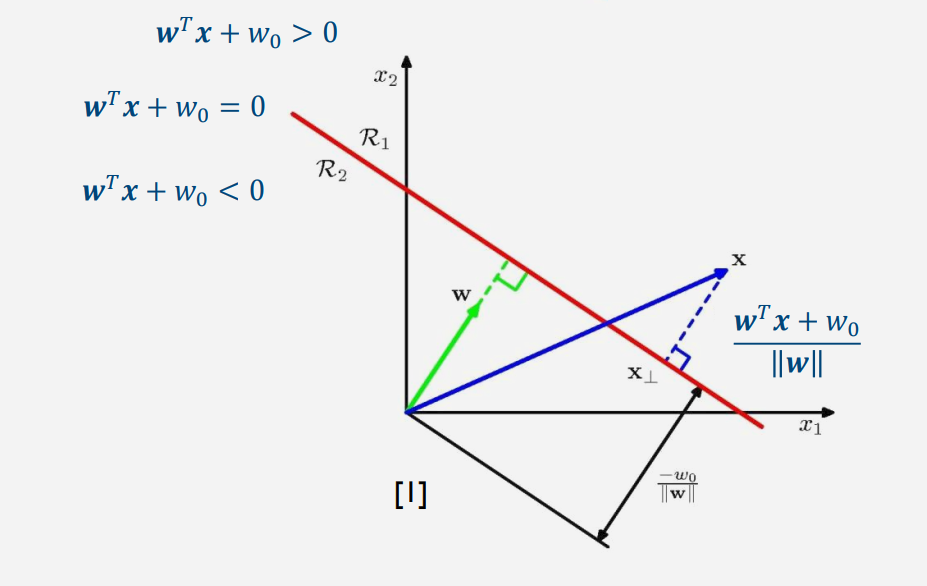
\includegraphics[width=0.5\linewidth]{image.png}
    \caption{مرز خطی جداکننده}
    \label{fig:enter-label}
\label{fig:f1}
\end{figure}

- سطح تصمیم (یا مرز تصمیم): \(w^Tx + w_0 = 0\) معادله‌ای است که مرز بین دو کلاس را مشخص می‌کند. این سطح یا خط، نواحی تصمیم را در فضای ویژگی جدا می‌کند، به طوری که نمونه‌هایی که در یک طرف این مرز قرار دارند به یک کلاس و نمونه‌هایی که در طرف دیگر قرار دارند به کلاس دیگر تعلق دارند.

\begin{figure}
    \centering
    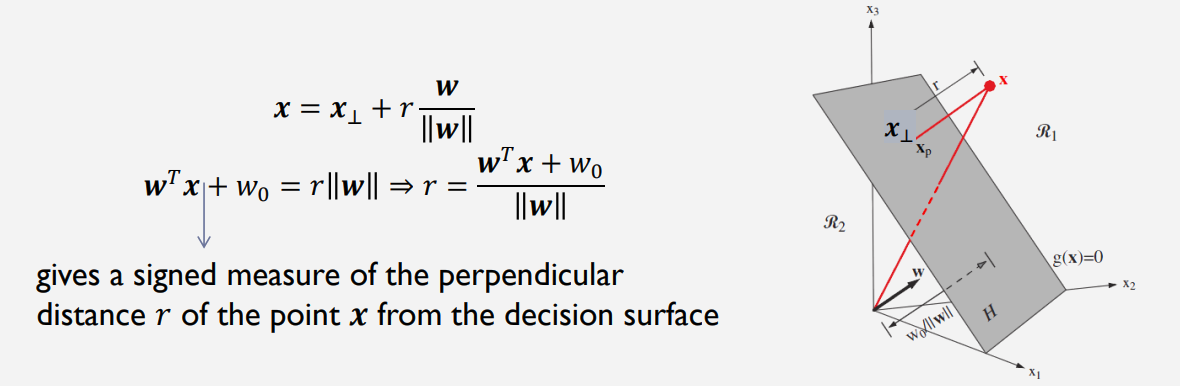
\includegraphics[width=1\linewidth]{image2.png}
    \caption{مرز جداکننده در داده‌های سه بعدی}
    \label{fig:enter-label}
\label{fig:f1}
\end{figure}

 \subsection{
$Cost\:function$ }

برای طبقه‌بندی‌کننده‌های خطی، تابع هزینه به شکل یک مسئله بهینه‌سازی تعریف می‌شود:

- ابتدا باید معیاری برای اندازه‌گیری خطای پیش‌بینی انتخاب شود.

- بر اساس مجموعه آموزشی \( D = \{(x^{(i)}, y^{(i)})\}^n_{i=1} \)، تابع هزینه \( J(w) \) تعریف می‌شود که در آن \( x^{(i)} \) نمونه‌های ورودی و \( y^{(i)} \) برچسب‌های مرتبط با این نمونه‌ها هستند.

- سپس، مسئله بهینه‌سازی حاصل برای یافتن بهترین پارامترها حل می‌شود: پارامترهای بهینه \( \hat{w} \) از طریق مینیمم کردن تابع هزینه \( J(w) \) بدست می‌آیند، یعنی \( \hat{w} = \arg\min_w J(w) \).

- معیارها یا توابع هزینه برای طبقه‌بندی به عنوان شاخصی از کیفیت طبقه‌بندی‌کننده خطی عمل می‌کنند و در اینجا چندین تابع هزینه برای مسئله طبقه‌بندی بررسی خواهند شد.
\subsubsection{$SSE$}

\[ J(w) = \sum_{i=1}^{N} (w^T x^{(i)} - y^{(i)})^2 \]

، تابع هزینه $Sum\:of\:Squared\:Errors\:(SSE)$ برای مسائل طبقه‌بندی مناسب نیست. علت این امر آن است که $SSE$ حتی برای پیش‌بینی‌هایی که "بیش از حد صحیح" هستند و در طرف صحیح تصمیم (خط تصمیم) قرار دارند، جریمه‌هایی اعمال می‌کند. در واقع، این تابع هزینه فاصله پیش‌بینی‌های صحیح را از خط تصمیم نیز به عنوان خطا تلقی می‌کند، که این موضوع در مسائل طبقه‌بندی مطلوب نیست. 

که در این فرمول \( w \) بردار وزن‌ها، \( x^{(i)} \) نمونه $i$-ام و \( y^{(i)} \) برچسب واقعی نمونه $i$-ام است. 
\begin{figure}
    \centering
    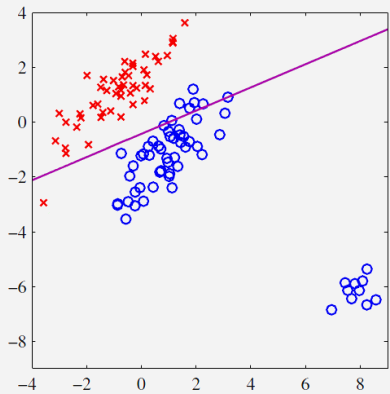
\includegraphics[width=0.5\linewidth]{image3.png}
    \caption{دسته بند دوتایی}
    \label{fig:enter-label}
\end{figure}
\end{document}
